\chapter{Introduction}
\label{CHAP_FIRST}
\centerline{\rule{149mm}{.02in}}
\vspace{2cm}

This section will outline an introduction to the project, discussing a number of different topics such as: 

\begin{itemize}
\itemsep0em
  \item The chosen domain and involved technologies
  \item The motives and justification behind the project
  \item The Aims and Objectives of the project
  \item The chosen approach to the execution of the project
  \item The Project Plan going forward
\end{itemize}

Hopefully, these explanations will give some context to the work being done, answering such questions as "Why this project?" and "What value does this work bring?"

\section[Overview]{Project Overview}

I chose to pursue this project for a number of reasons. Firstly, Cloud Computing is an area of technology which I have great interest in, having worked with similar technologies in previous employment and in personal projects. Secondly, and perhaps more importantly, is the incredible rise of the Cloud to prominence in the Computing industry in recent years, with the Infrastructure as a Service (IaaS) model at the forefront. The emergence of public clouds from tech giants such as Amazon and Microsoft has lead to a huge increase in the popularity of related software technologies, usually Virtual Infrastructure Managers using Virtualisation technology to service clients' computing needs in an on-demand manner. \\ 
Amongst the many current solutions out there, one technology in particular has grown in popularity to the point that it is fast becoming the de facto open source standard for IaaS clouds. This technology is OpenStack. 
This popularity makes OpenStack a perfect candidate to be assessed in terms of its capabilities and characteristics; in short, we want to know  \textit{why} OpenStack is becoming so popular, and if this popularity is justified.  
In order to answer this question, my work will involve researching into the relevant areas of Cloud Computing, Data Centre Virtualisation and Web Services, and performing qualitative and quantitative assessment of OpenStack through various approaches and experiments. 

\subsection{Project Aims and Justification}

There are a number of aims to this project. Firstly, I aim to research the area of Infrastructure as a Service Clouds, including the desirable characteristics and requirements of these clouds from a number of different perspectives, current IaaS market offerings, and what technologies are involved in producing such a solution. This research should culminate in an overview of OpenStack, which technologies it uses, and what it does. Once this background research preparation is complete, my main target will be to produce a critical evaluation of OpenStack, in the form of a report, detailing OpenStack with respect to its functionality and architecture. I also aim to perform both qualitative and quantitative assessment of OpenStack through experiments. These experiments will also be part of my deliverable, and should serve as documentation of how to use OpenStack, and provide re-usable software to test the functionality of OpenStack. The results of these experiments will be used as evaluation. Finally, I will analyse my results and approach to evaluation of OpenStack, and ask a number of questions concerning how well my performance covers the technology, how reliable my results are, and what impact my evaluation actually has. This evaluation of my evaluation will serve as another deliverable, giving an assessment of the advantages and disadvantages of my approach in retrospect.  \\ 
I consider this project to be worthwhile mainly due to the importance of OpenStack, considering its relative infancy in the market compared to it's competitors. This product is becoming increasingly dominant, and yet was only released in 2010 \cite{Piatt10}, so much less is known about it than many other solutions. For this reason, I believe an analysis of the product is worthwhile. Secondly, this project serves as a precursor for an EU project, ASCETiC \cite{ascetic}, which the School of Computing will be involved with; The knowledge and guides provided by this project could be very helpful in the workings of the project. This backing alone justifies the idea of getting to know OpenStack better. 

\subsection{Objectives}

Formally, my objectives are as follows:
\begin{itemize}

\item \underline{Produce a Literature Review of relevant source material}: A background research report, starting with Cloud Computing as a whole, with particular focus on public clouds, virtualisation, IaaS and the current IaaS market, and of course, OpenStack. The idea behind this is to give context to the reader and introduce them to the various technologies and concepts involved in this project. 

\item \underline{Produce an Evaluation Report of OpenStack}: The main deliverable of this project, the report will provide guides of how to use OpenStack, useful for future projects, as well as providing insight as to the workings of OpenStack via Qualitative \& Quantitative assessment. The report will draw conclusions about OpenStack as a whole, and give some idea of whether it is a good idea to use it. 

\item \underline{Produce a number of designed experiments and results to assess OpenStack functionality}: will be varied, so as to assess OpenStack in a number of different ways. The experiments should be designed, implemented, and then executed, with results and derived conclusions attached. They will serve as a source of information for the Evaluation report. 

\item \underline{Produce Implementations for a number of programmatic tests of OpenStack}: This objective is closely linked to the previous objective. Some experiments will be programmatic tests written using the various RESTful Web Services provided by OpenStack. These should be able to be reused given a different endpoint for the Web Service Client, and so full implementations of these should be provided as a deliverable. They will also be used to validate OpenStack functionality. 

\item \underline{Produce re-usable software components for use of OpenStack}: Similarly to the previous objective, a set of software tools should be produced as part of this project, which will allow others to easily interact with OpenStack in the same way this project has for experiments. This will most likely be a Java tool, providing access to OpenStack's APIs. 

\item \underline{Produce an evaluation of my approach to evaluating OpenStack}: The final objective is to provide some evaluation of my work. This is a way of comparing my evaluation with others that are out there, and assessing the successes and shortcomings of my approach and work. I will discuss how I may have improved my approach in this part of the report, and how this would have improved the outcome. I will also assess the quality of my deliverables.   

\end{itemize}

\subsection{Minimum Requirements}

The minimum requirements of this project to achieve a pass are as follows:
\begin{itemize}
\itemsep0em

\item Provide a \underline{basic literature review} of Cloud Computing, Virtualisation, IaaS and OpenStack. 
\item Provide at least 1-3 repeatable \underline{designed experiments} to assess the functionality of OpenStack, with logs and results. 
\item Provide code for at least one \underline{programmatic experiment} to assess the functionality of OpenStack, with source code, logs and results. 
\item Provide an \underline{Evaluation Report} of OpenStack containing Qualitative Assessment of its features. 
\item Provide at least one \underline{re-usable software component} for OpenStack. 
\item Produce an \underline{Evaluation} of the project approach. 

\end{itemize}

\subsection{Possible Extensions}

There are a number of possible extensions to this project which could be performed if there is enough time. These are extensions that are not expected to be completed, and are beyond even exceeding the minimum requirements, and achieving all of the stated objectives. Extensions are listed below:
\begin{itemize}
\itemsep0em
\item \underline{Comparison with another product} - deploy an alternative cloud computing platform, in order to gain perspective particularly with respect to quantitative results. 
\item \underline{Different OpenStack configurations} - perform experiments with a number of different OpenStack setups; 
\item \underline{Produce an experiment/test framework} - provide some reusable code to create new experiments for OpenStack; this could just be a set of commonly used utilities, or a fully blown programming/testing framework. 
\end{itemize}

\subsection{Deliverables}

These are the deliverables of the project, based on the minimum requirements. 
\begin{itemize}
\itemsep0em
\item \underline{An Evaluation Report} - detailing strengths and weaknesses of OpenStack
\item \underline{Designed Experiments} - with descriptions, targeting functionality of OpenStack
\item \underline{Logs \& Results} - From aforementioned experiments, including code from programmatic tests. 
\item \underline{Re-usable software components} - For future interaction with OpenStack, could be scripts, programming libraries, etc.
\item \underline{Evaluation} - Of the project approach, where it succeeded and failed, and other critical points.
\end{itemize}

\section{Methodology}
\subsection{Project}
In order to achieve the objectives set for this project, work will be split into 4 key areas. These areas are left deliberately wide and high level so as to allow an agile, iterative approach to development. The key reason for this approach is my inexperience with the software and technologies involved, and the time constraints. It is likely that much learning of OpenStack will commence whilst the experiments are being developed, and this new knowledge could have an effect on how the experiments are written. For this reason, a traditional waterfall model with clearly separated stages such as 'design' and 'implementation' would not be ideal. \\
The three steps are as follows:
\begin{enumerate}
\itemsep0em
\item \underline{Research Phase} - concerned with laying the ground work of the project, including literature review \& project planning.
\item \underline{Implementation Phase} - covers most of the practical work, stretching from initial design of the experiments to the logging of results from executing those experiments. 
\item \underline{Conclusion phase} - Once all data has been collated and collected, conclusions must be made regarding the work done, and the evaluation itself must be summed up.
\item \underline{Evaluation Phase} - Every stage of the process must be evaluated. This phase is chiefly for writing up this evaluation, as the plan is to constantly evaluate work at each stage of the project. 
\end{enumerate}  
Version control will be used for all code including write up, and tasks will be managed through the use of productivity tools such as note taking applications, and code comments. 

\subsection{Experiment}

Development of experiments will follow an iterative model, allowing for an agile approach. This is mainly due to it being likely that each experiment will adapt and change as I become more comfortable with OpenStack, and with the technologies involved. If experiments have some practical element, e.g. programming, and require development of some deliverable, they will roughly follow an agile design-implement-test cycle, until the results are deemed reliable. Development will happen mostly in 'sprints' bursts of work with dedicated outcome objectives.\\
In terms of the types of experiment, a mixed approach of Quantitative and Qualitative experiments are likely to be developed. Qualitative experiments are those producing qualitative results, i.e. those which cannot be expressed as a number\cite{qualquantdef}. For example, when comparing features, whether OpenStack has a feature is qualitative. Quantitative experiments are those producing quantitative results, i.e. those which can be quantified, or expressed as a number\cite{qualquantdef}. For example, performance tests of a task with OpenStack may give numerical time results - these are quantitative. \\
Combining these two approaches could give a more well-rounded evaluation, based both on its performance and characteristics. This will be elaborated on in the literature review. 

\section{Project Plan}
In this section, the plan for the project will be set out, including the work schedule and the various milestones of the project. This structure is put in place to allow a more methodical and organised approach to the project work. 

\subsection{Schedule}

This project will follow a specific schedule on a weekly basis, proposed in the first week of the project, hopefully allowing for a structured set of goals every week. This of course is difficult to predict in any project, and any changes to the proposed schedule will be discussed in the Evaluation section of this report.  

\subsection{Milestones}

Milestones are important in a project in that they give a good indication on how far along the project is, and set a clear target on when goals should be achieved. These are listed below:

\begin{itemize}
\itemsep0em
\item \underline{Milestone 1} - The minimum requirements \& aims and objectives must be agreed on and delivered in week 2 (7th February 2014). 
\item \underline{Milestone 2} - The literature review first draft must be completed by week 5 (2nd March 2014) to allow for practical work to commence. 
\item \underline{Milestone 3} - The mid-project report must be delivered on 7th March 2014. Some evidence of work with OpenStack must be seen by then. 
\item \underline{Milestone 4} - At least 2 experiments must be designed and executed by week 11 so as to begin writing up the results. 
\item \underline{Milestone 5} - The progress meeting will take place on 30th April 2014. This is a demonstration of the project to supervisor and assessor. 
\item \underline{Milestone 6} - This report must be submitted by 14th May 2014. 

\end{itemize}

\subsection*{GANTT Chart}

An initial GANTT Chart detailing the aforementioned schedule \& milestones is provided, along with a chart of project deadlines, in Appendix F. 

%\begin{figure}[ht]
%\centering
%\fbox{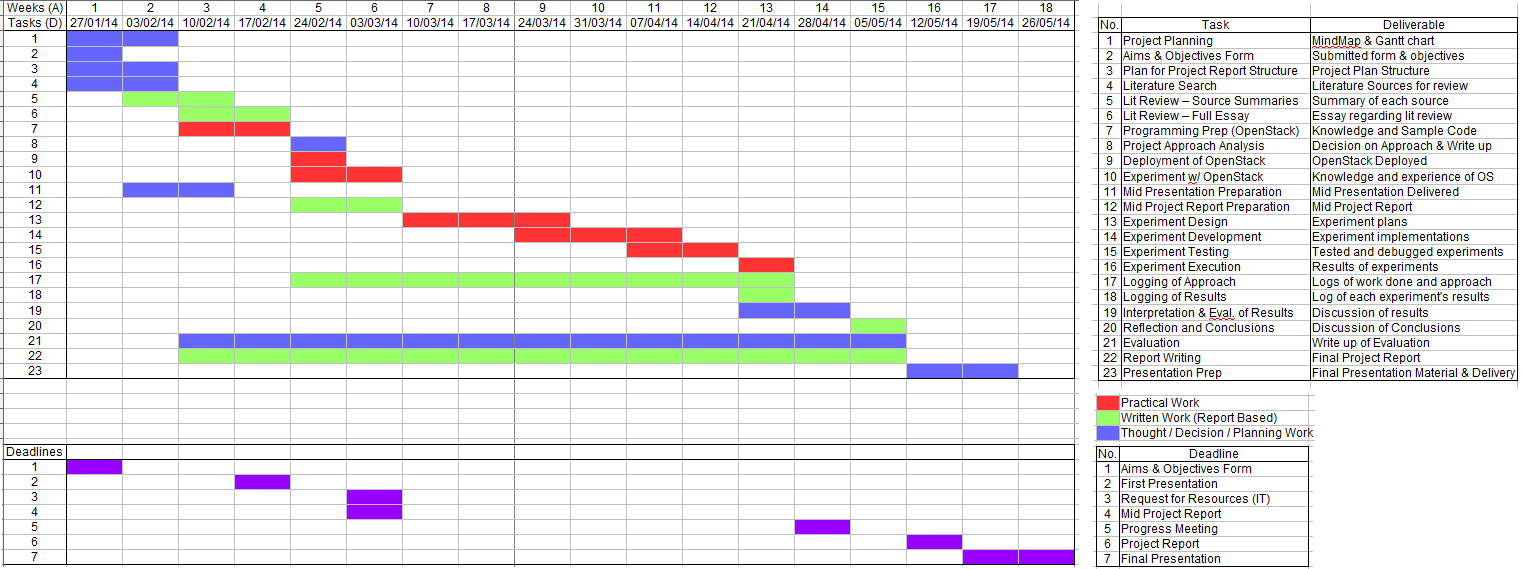
\includegraphics[scale=0.44]{joint-gantts3}}
%\caption{GANTT Chart representing initial project schedule \& Deadlines}
%\end{figure}
\section{Conclusion}

In this section, the fundamental basis of the problem \& subsequent project, as well as the approach to be taken, have been described. Certain aspects of project management have also been covered, to give some idea of how the work will be executed. At this point, the reader should have some idea of what this project is trying to achieve and why, and also some idea of how it will be completed. \\

In the next section, to continue with the 'build up' to the project work, the various aspects of technology which are relevant to the project will be researched and laid out for the reader, in order to build up an understanding of the project domain and its various concepts. The section will also consider, based on the knowledge acquired, how to proceed with an 'Evaluation of OpenStack' beyond a high level project approach. 